\documentclass{standalone}

\usepackage{tikz}
\usetikzlibrary{decorations.pathreplacing}
\usetikzlibrary{positioning}

\begin{document}
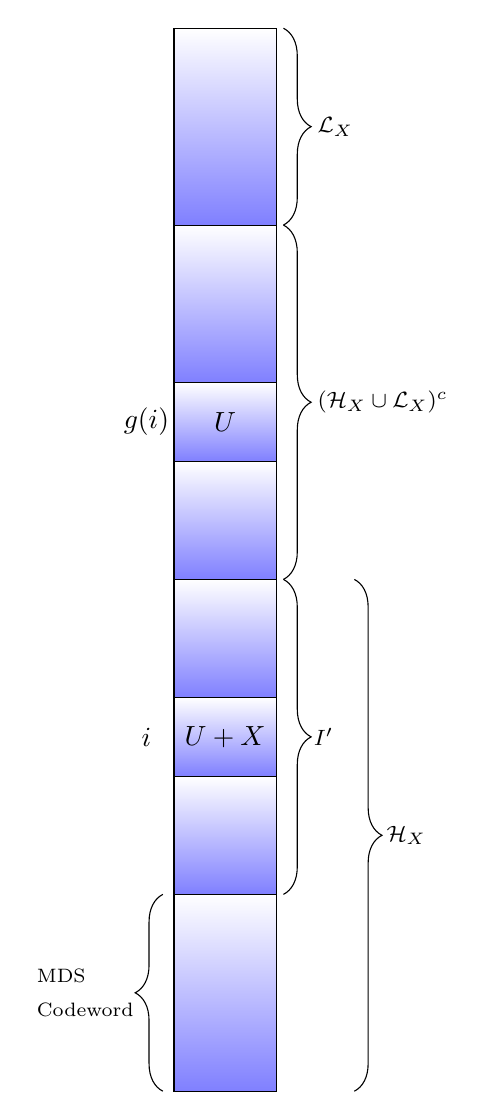
\begin{tikzpicture}

    \filldraw[top color=white,bottom color=blue!50!] (0.5,0) rectangle node{} +(1.3,2.5);
    \draw [decorate,decoration={brace,amplitude=10pt},xshift=-4pt,yshift=0pt]
    (0.5, 0) -- (0.5, 2.5) node [black,midway,xshift=-0.6cm, text width=2cm, align=left] 
    {\scriptsize MDS\\ Codeword};
    \filldraw[top color=white,bottom color=blue!50!] (0.5, 2.5) rectangle node{} +(1.3, 1.5);
    \filldraw[top color=white,bottom color=blue!50!] (0.5, 4.0) rectangle node (UX) {$U+X$} +(1.3, 1);
    \draw node[left of=UX] {$i$};
    \filldraw[top color=white,bottom color=blue!50!] (0.5, 5.0) rectangle node{} +(1.3, 1.5);
    \filldraw[top color=white,bottom color=blue!50!] (0.5, 6.5) rectangle node{} +(1.3, 1.5);
    \draw [decorate,decoration={brace,amplitude=10pt,mirror,raise=4pt},yshift=0pt]
    (1.75, 2.5) -- (1.75, 6.5) node [black,midway,xshift=0.65cm] {\footnotesize
    $I'$};
    \draw [decorate,decoration={brace,amplitude=10pt,mirror,raise=4pt},yshift=0pt]
    (2.65, 0) -- (2.65, 6.5) node [black,midway,xshift=0.8cm] {\footnotesize
    $\mathcal H_{X}$};
    \filldraw[top color=white,bottom color=blue!50!] (0.5, 6.5) rectangle node{} +(1.3, 1.5);
    \filldraw[top color=white,bottom color=blue!50!] (0.5, 8.0) rectangle node (U) {$U$} +(1.3, 1);
    \draw node[left of=U] {$g(i)$};
    \filldraw[top color=white,bottom color=blue!50!] (0.5, 9.0) rectangle node{} +(1.3, 2);
    \filldraw[top color=white,bottom color=blue!50!] (0.5, 11.0) rectangle node{} +(1.3, 2.5);
    \draw [decorate,decoration={brace,amplitude=10pt,mirror,raise=4pt},yshift=0pt]
    (1.75, 6.5) -- (1.75, 11.0) node [black,midway,xshift=1.4cm] {\footnotesize
    $( \mathcal H_{X} \cup \mathcal L_{X} )^{c}$};
    \draw [decorate,decoration={brace,amplitude=10pt,mirror,raise=4pt},yshift=0pt]
    (1.75, 11.0) -- (1.75, 13.5) node [black,midway,xshift=0.8cm] {\footnotesize
    $\mathcal L_{X}$};
\end{tikzpicture}

\end{document}
